\subsection{Handicaps}

Les Handicaps représentent les défauts qui compliquent parfois la vie de votre personnage. Certains sont plus contraignants que d’autres et certains dépendent du scénario. Ils permettent de choisir des Atouts supplémentaires mais surtout ajoutent du caractère à votre personnage et augmente ainsi son intérêt et votre plaisir de jouer.

\begin{description}[align=left]
    \item [Âgé (Majeur)]
        Votre héros se fait vieux, certes, mais n’est pas encore prêt pour l’hospice. Son Allure est réduite de 1. Sa Force et sa Vigueur diminuent d’un type de dé (selon l’age, minimum d4). Elles ne pourront plus jamais être élevées. Le côté positif, c’est que l’expérience de l’âge lui rapporte 5 points de Compétences supplémentaires à répartir sur toutes Compétences liées à l’Intellect.

    \item [Anémique (Mineur)]
        Votre héros est particulièrement sensible aux maladies, à la fatigue et aux effets de l’environnement. Il subit un malus de -2 à tous les jets de Vigueur pour résister à la fatigue, au poison, aux maladies, etc\ldots

    \item [Arrogant (Majeur)]
        Votre héros ne pense pas qu’il est le meilleur, il le sait. Quel que soit le domaine, nul ne peut le battre et il le prouve à chaque occasion. Gagner ne lui suffit pas. Il doit totalement dominer son adversaire. Si un adversaire doute de sa supériorité, il cherchera à l’humilier et à lui prouver qu’il peut le battre quand il veut.\\
        Les héros Arrogants cherchent toujours le chef adverse dans un combat, n’attaquant ses subalternes que s’ils se mettent en travers de leur chemin.

    \item [Aveugle (Majeur)]
        Votre héros est complètement aveugle. Il subit un malus de -6 à toutes les tâches nécessitant la vue (à peu près toutes ou presque) et -2 à toutes les interactions en société (il ne peut pas déchiffrer les expressions de ses interlocuteurs). Le bon côté, c’est que les personnages Aveugles obtiennent un Atout supplémentaire de leur choix pour compenser ce Handicap particulièrement pénalisant.

    \item [Bavard (Mineur)]
        On dit qu’une grande gueule peut couler un navire. Votre héros l’est au point qu’il pourrait couler une armada. Il ne sait pas garder un secret, il dévoile tous les plans et même les secrets les mieux gardés de ses amis et choisit toujours le plus mauvais moment pour le faire.

    \item [Bizarrerie (Mineur)]
        Votre héros possède une bizarrerie, rien de grave, mais pouvant lui causer des ennuis. Un escrimeur qui tente d’abord de zébrer ses initiales sur ses ennemis avant de les attaquer, un droïde de protocole se vantant sans cesse de sa culture ou une jeune snob qui refuse de s’asseoir, boire ou manger avec les gens de classe inférieure sont tous des exemples bizarrerie.

    \item [Boiteux (Majeur)]
        Une vieille blessure a presque estropié votre héros. Son Allure est réduite de 2 et il n’utilise qu’un d4 pour courir. L’Allure d’un personnage ne peut jamais passer en dessous de 1.

    \item [Borgne (Majeur)]
        Votre héros a dans le passé eu l’\oe{il} crevé par un ennemi. S’il ne porte pas un bandeau ou un \oe{il} de verre (d’un prix de l’ordre de 500 Cr) il subit -1 à son Charisme à cause de sa vilaine blessure. Il subit -2 à tout jet de Trait nécessitant une perception de la profondeur (Tirer, Lancer, sauter d’un bâtiment à l’autre et ainsi de suite).

    \item [Chimères (Mineur ou Majeur)]
        Votre héros croit en des choses qui paraissent étranges pour les autres. Les Chimères Mineures sont inoffensives ou alors le personnage y fait rarement allusion (les chiens parlent, on est tous des personnages d’un jeu bizarre, etc\ldots).\\
        Avec une Chimère Majeure, il exprime souvent ses opinions sur le sujet et cela peut s’avérer dangereux (je suis allergique aux armures, les Vong sont mes amis, etc\ldots).

    \item [Couard (Majeur)]
        Tout le monde n’a pas des nerfs d’acier. Votre héros blêmit à la vue du sang et est terrifié à l’idée même de subir une blessure. Tous ses tests de terreur subissent un malus de -2.

    \item [Code d’Honneur (Majeur)]
        L’honneur est très important aux yeux de votre personnage. Il n’a qu’une parole, traite ses prisonniers avec décence et se conforme d’ordinaire aux codes de bonne conduite et règles de bienséance de son monde.

    \item [Cupide (Mineur)]
        Votre héros est un grippe-sou qui mesure sa valeur en trésor.

    \item [Curieux (Majeur)]
        C’est un vilain défaut et votre personnage est très vilain. Les personnages Curieux sont facilement attirés par l’aventure. Il faut qu’ils fouillent partout et désirent toujours savoir ce qui se cache derrière chaque mystère.

    \item [Deux mains gauches (Mineur)]
        Certaines personnes ne sont tout simplement pas douées avec la technologie. Un personnage affligé de ce défaut subit systématiquement un malus de -2 à ses jets de Réparer. Et chaque fois qu’il utilise un appareil technologique, un résultat de 1 sur son dé de Compétence (sans tenir compte du dé Joker) signifie que l’appareil se détraque. Le remettre en état nécessitera un jet de Réparer à -2 et 1d6 heures de travail.

    \item [Dur d’Oreille (Mineur ou Majeur)]
        Un personnage ayant perdu tout ou partie de son acuité auditive possède ce Handicap. Un Handicap Mineur fait subir -2 à tous ses jets de Perception liés à l’audition y compris se réveiller à cause du bruit. Un Handicap Majeur signifie que le personnage est sourd et rate automatiquement tous ses jets de Perception liés à l’audition.

    \item [Ennemi (Mineur ou Majeur)]
        Quelqu’un quelque part déteste votre héros et veut sa mort. Le niveau du Handicap dépend de la puissance de l’ennemi et de sa fréquence d’apparition. Un Ennemi Mineur sera un chasseur de prime solitaire avide de vengeance. Un Ennemi Majeur sera un seigneur Sith démoniaque vouant une haine implacable envers votre héros.\\
        Si l’Ennemi est vaincu le MJ s’arrange pour lui trouver un remplaçant à moins que le héros n’efface le Handicap en sacrifiant une Progression.

    \item [Étranger (Mineur)]
        Votre héros n’appartient pas à la société dans laquelle il vit. Un Wookie sur Ryloth, un Gungan au sénat, etc\ldots Les marchands augmentent leurs prix pour le personnage, lui refusent leur aide et le traitent comme s’il était d’un rang inférieur. \\
        En plus des effets de roleplay ci-dessus, le Charisme de votre héros subit tout le temps un malus de -2, sauf quand il est parmi ses semblables.

    \item [Frêle (Majeur)]
        Votre héros est soit très petit, soit très maigre, voire les deux par rapport à la norme de son peuple. Sa Résistance est réduite de 1 à cause de sa faible stature.

    \item [Mal de l’espace (Mineur)]
        Votre héros ne supporte pas les voyages à vitesse super luminique. Quelque chose dans les déplacements en hyperespace le rend malade. Après chaque déplacement hyperespace, il souffre d’un niveau de fatigue pendant 24h. Les voyages en hyperespace peuvent l’affaiblir mais pas le tuer.

    \item [Gamin (Majeur)]
        Il arrive que des événements incroyables poussent des enfants vers l’aventure. Sachez que choisir ce Handicap signifie débuter avec un gros désavantage. Les héros Gamins ont entre 8 et 12 ans (en âge humain. Adaptez en fonction des races où les tranches d’âge sont différentes). Ils ne disposent que de 3 points à investir dans leurs Attributs et de 10 points dans leurs Compétences.\\
        Le bon côté de la chose, c’est que les Gamins ont beaucoup de chance. Ils débutent chaque session de jeu avec un Jeton en plus. Ce dernier est cumulable avec les autres Jetons attribués par les Atouts Chanceux ou Très Chanceux. Quand votre héros arrive à maturité, ce Handicap disparaît naturellement. Il en a déjà bien payé le prix. Il n’obtient plus non plus le Jeton offert par le Handicap lorsqu’il atteint l’âge de 18 ans (ou équivalent pour une autre race).

    \item [Héroïque (Majeur)]
        Votre héros ne dit jamais non à une personne dans le besoin. Cela peut ne pas lui plaire mais il se sent obligé de secourir ceux qu’il considère sans défense. C’est le premier à se jeter dans un immeuble en flammes, à accepter de chasser les monstres pour trois fois rien et ne pas savoir résister aux larmes d’une belle infortunée.

    \item [Ignorant (Majeur)]
        Votre héros en sait moins que les autres sur le monde dans lequel il vit. Il subit un malus de -2 aux jets de Culture générale.

    \item [Illettré (Mineur)]
        Votre héros ne sait pas lire. Il peut écrire son nom et sait ce qu’un panneau STOP signifie, mais c’est à peu près tout. Les maths ne sont pas son fort non plus. 2 + 2 = 4 passe encore mais ne lui parlez pas de multiplication. Les Illettrés ne savent ni lire, ni écrire, quel que soit par ailleurs le nombre de langues qu’ils savent parler.

    \item [Loyal (Mineur)]
        Votre personnage n’est peut-être pas l’archétype du héros, mais il donnerait sa vie pour ses amis. Il est incapable de laisser tomber ses compagnons s’il a la moindre possibilité de leur venir en aide.

    \item [Malchanceux (Majeur)]
        Votre héros est moins chanceux que les autres. Il reçoit un Jeton de moins par session de jeu. Un héros ne peut être Malchanceux et Chanceux à la fois.

    \item [Manchot (Majeur)]
        Votre héros est né avec un seul bras ou l’a perdu lors d’un combat passé. Fort heureusement, il lui reste l’autre, le bon. Il subit un malus de -4 pour les tâches qui requièrent deux bras comme Escalade par exemple.

    \item [Mauvaise habitude (Mineur ou Majeur)]
        Votre héros possède une manie grossière et porte sur les nerfs de son entourage. Il se cure le nez, dit « t’sais » à chaque phrase ou bien mâche son chewing-gum en permanence. Une Mauvaise habitude Mineure irrite son entourage mais n’est pas dangereuse. Son Charisme est réduit de 1.

        Une Mauvaise habitude Majeure représente une dépendance avilissante voire mortelle. Cela englobe drogues, alcool ou être accro à une activité associale. Un héros privé de sa dose fait un jet de fatigue toutes les 24h. Le premier jet manqué le rend Fatigué, puis Épuisé. Le stade final est le coma pour l’usage de drogues ou des troubles du comportement pour l’alcool ou les autres activités.

        Des soins médicaux apaisent les symptômes, sinon il doit vivre avec les malus durant 1d6 jours. Par la suite le héros peut effacer le Handicap en échange d’une Progression sinon il rechute dans sa dépendance.

    \item [Moche (Mineur)]
        La nature n’a pas été tendre concernant l’apparence de votre héros. Son Charisme est réduit de 2 et il est généralement rejeté par les membres du sexe opposé.

    \item [Myope (Mineur)]
        La vue de votre héros n’est plus ce qu’elle était. Avec des lunettes il ne subit aucune pénalité et le Handicap est Mineur. S’il perd ses lunettes (50\% de chance que cela arrive lorsqu’il est blessé et aucune si les lunettes sont attachées), il subit -2 à tous ses jets de Trait pour Tirer ou Percevoir quelque chose situé à plus de 5 cases (10 mètres).

    \item [Obèse (Mineur)]
        Les personnes corpulentes éprouvent rapidement de grandes difficultés lors des situations physiques dangereuses. Ceux qui ne souffrent pas de leur corpulence ont l’Atout Costaud. Ceux qui en souffrent sont Obèses. Un personnage ne peut être Costaud et Obèse. Un Obèse ajoute 1 à sa Résistance, réduit de 1 son Allure et il utilise un d4 pour courir. Il aura en outre du mal à trouver des vêtements ou des armures à sa taille, à rentrer dans des lieux exigus ou encore voyager avec un speeder par exemple.

    \item [Pacifiste (Mineur ou Majeur)]
        Votre héros déteste la violence. Un Pacifiste Mineur ne se bat que lorsqu’il n’a pas d’autre choix et n’accepte pas le meurtre de prisonniers ou de victimes sans défenses. 

        Un Pacifiste Majeur ne combattra aucun être vivant dans aucune circonstance. Il peut se défendre, mais ne fera jamais rien qui puisse blesser une créature vivante ou pensante. 

        À noter que n’entrent pas dans cette catégorie les êtres maléfiques, les Sith. Un Pacifiste Majeur pourra éventuellement combattre en utilisant des techniques non létales (comme ses poings par exemple). Ce type de personnage ne prendra de telles mesures drastiques que si sa vie en dépend.

        Un Apprenti Sith ou un Seigneur Sith ne peut avoir ce Handicap. Ce handicap peut être effacé contre 1 progression.

    \item [Phobie (Mineur ou Majeur)]
        Les Phobies sont des peurs irrationnelles qui empoisonnent le héros pour le reste de sa vie. Chaque fois qu’il est en présence de sa Phobie, il subit -2 à tous ses jets de Traits si c’est un Handicap Mineur et -4 s’il est Majeur. 

        Les Phobies ne doivent pas être trop évidentes. Tout le monde à peur de mourir donc il ne s’agit pas d’une Phobie, mais simplement de bon sens. L’objet d’une Phobie devrait être un élément anodin sur lequel son esprit s’est fixé durant une rencontre qui a produit cette frayeur.

        Et souvenez vous, les Phobies représentent des peurs irrationnelles.

    \item [Poches percées (Mineur)]
        Le dicton dit qu’un idiot et son argent ne font pas bon ménage. Votre héros est l’idiot en question. Il débute avec la moitié des fonds usuels. Il a du mal à économiser ce qu’il gagne. Chaque semaine de jeu environ, son joueur divise ses fonds par deux.

    \item [Prudent (Mineur)]
        Ce personnage incarne l’extrême prudence. Il ne prend aucune décision hâtive, a besoin du maximum d’informations et de peaufiner le moindre détail avant d’agir.

    \item [Présomptueux (Majeur)]
        Rien ne peut résister à votre héros. C’est du moins ce qu’il croit. Il se croit capable de tout faire et ne recule devant aucun défi. Il n’est pas suicidaire mais il prend des risques en dépit du bon sens.

    \item [Rancunier (Mineur ou Majeur)]
        Votre héros n’oublie jamais les offenses qui lui sont faites. En Handicap Mineur, il se venge par des moyens légaux. En Handicap Majeur il ira même jusqu’au meurtre pour se venger d’un affront.

    \item [Recherché (Mineur ou Majeur)]
        Votre héros a commis un crime dans son passé et sera arrêté s’il est repris par les autorités. Le niveau du Handicap dépend de la gravité du crime. Une note de bar impayé constituera un Handicap Mineur, tout comme un héros recherché pour des crimes plus sérieux mais vivant loin des lieux du délit. \^Etre accusé de trahison ou de rébellion envers l’empire sont des crimes plus sérieux.

    \item [Rien à perdre (Mineur)]
        N’avoir Rien à perdre ne signifie pas que votre héros est suicidaire mais qu’il ne tient à la vie que pour atteindre un but qu’il s’est fixé. Peut-être veut-il venger sa famille massacrée ou finir en beauté car il est condamné par une maladie.

        Il ne risquera pas sa vie sans raisons valables, mais si l’occasion de réaliser son but se présente, il fera n’importe quoi et prendra tous les risques pour parvenir.

    \item [Sale caractère (Mineur)]
        Votre héros est désagréable et a très mauvais caractère. On ne l’apprécie pas beaucoup et il fait rarement preuve de gentillesse. Il fait payer le moindre des services qu’il rend et va jusqu’à faire la grimace quand on le récompense pas. Son Charisme est réduit de 2.

    \item [Sanguinaire (Majeur)]
        Votre héros ne fait jamais de prisonniers à moins d’être sous la surveillance étroite d’un supérieur. Cela peut causer de gros problèmes lors d’une campagne militaire sauf si vos supérieurs approuvent un tel comportement. Le Charisme de votre héros est réduit de 4 si sa cruauté de sa conduite est un fait connu de tous.

        Ce handicap n’est pas compatible avec les atouts Padawan et Maître Jedi.

    \item [Sceptique (Mineur)]
        Les Sceptiques ne croient en la Force que quand ils y sont directement confrontés et même dans ce cas ils se raccrochent à la raison, se persuadant du contraire ou en ignorant purement l’évidence.

        Les Sceptiques subissent un malus de -2 à leurs tests de terreur lorsqu’ils sont confrontés à la Force.

    \item [Serment (Jedi ou Sith) (Majeur)]
        Le personnage a prêté serment il ne peut s’y soustraire. Voir la section sur La~Force~\ref{sec:force-serment} (p.~\pageref{sec:force-serment}).

    \item [Têtu (Mineur)]
        Votre héros veut toujours avoir raison et n’admettra jamais ses torts. Même devant la preuve évidente de son erreur il continue à se justifier de toutes les manières possibles.

    \item [Unijambiste (Majeur)]
        Avec une béquille (ou une jambe de bois) ce Handicap fonctionne comme le Handicap Boiteux, l’Allure est réduite de 2 et le dé pour courir est un d4.

        Sans béquille l’Allure passe à 2 et il ne peut pas courir. Il subit aussi un malus de -2 à tous les jets qui nécessitent de la mobilité, comme Grimper et Combat. Un unijambiste subit aussi un malus de -2 à ses jets de Natation (et -2 à son Allure dans l’eau).

        Il est possible d’éliminer ce Handicap avec une prothèse mais ces dernières sont très chères (200 000 Cr).

\end{description}

\begin{paperbox}{Serment (Jedi / Sith)}
    Ce Handicap est pris d’office quand un personnage prend l’Atout Maître Jedi ou Seigneur Sith. Il représente le serment au code d’honneur de l’ordre auquel le personnage souhaite appartenir.

    Ce handicap oblige le joueur à suivre le code de son ordre à la lettre sous peine de succomber à la Force et de devenir incontrôlable (PNJ).

    Voir le chapitre sur La Force~\ref{sec:force-serment} (p. \pageref{sec:force-serment}) pour plus de détails.
\end{paperbox}

\newpage
\vspace*{\fill}
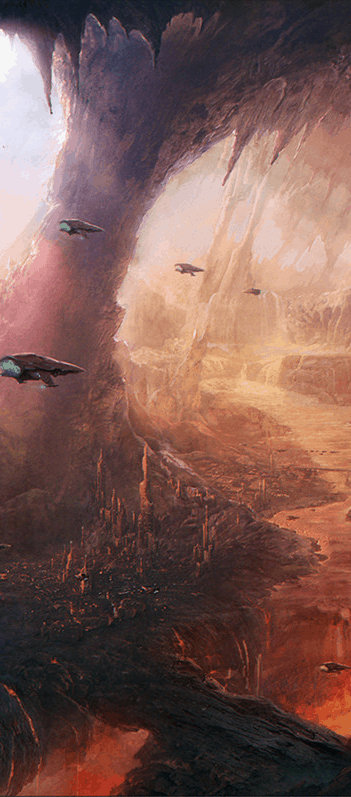
\includegraphics[width=\linewidth]{img/personnages/handicap.jpg}
